\section{Case Studies}
\label{sec:test}
In this chapter, we present two recognition systems working on the Poissonian subset as examples of using the NE15-MNIST dataset.
They provide possible concerns of creating benchmark tests, such as, using unified SNN description language, standard learning rules and neural models.
Thus, in order to apply the same benchmarking system on various simulators both software and hardware.
Evaluation on such a benchmark test is still under investigation, the case studies only give an attempt.

\subsection{Case Study I}
It is a simple two-layered network where the input neurons receive Poissonian presented spike trains from the dataset and forwards the connections to the decision neurons.
During the training, each decision neuron is triggered by a teaching neuron while the weights of the synaptic connections of the input neurons and the decision neuron are modulated with the standard STDP learning rule, see Fig~\ref{Fig:train}.
The model utilises Leaky-Integrate-and-Fire (LIF) neurons, and the parameters were all with biological means, see the listed values in Table~\ref{tbl:pynnSetting}.
The model is described with PyNN and the code is published in the same github repository.
Consequently, the benchmark model can be directly run on different SNN simulators as long as PyNN is supported.
Besides, any modification on neuron or learning model is not required since only standard models are used.

\begin{table}[hbbp]
\centering
\caption{\label{tbl:pynnSetting}Parameter setting for the current-based LIF neurons using PyNN}
\begin{tabular}{c|c|c}
\hline
Type & IF\_curr\_exp & Units\\
\hline
cm & 0.25 & nF	\\
%\hline
tau\_m & 20.0 & ms\\
%\hline
tau\_refrac & 2.0 & ms\\
%\hline
tau\_syn\_E & 1.0 & ms\\
%\hline
tau\_syn\_I & 1.0 & ms\\
%\hline
v\_reset & -70.0 & mV\\
%\hline
v\_rest & -65.0 & mV\\
%\hline
v\_thresh & -50.0 & mV\\
\hline
\end{tabular}
\end{table}

\begin{figure}[hbt!]
	\centering
	\subfloat[Training model of a single decision neuron.]{
		\label{Fig:train}
		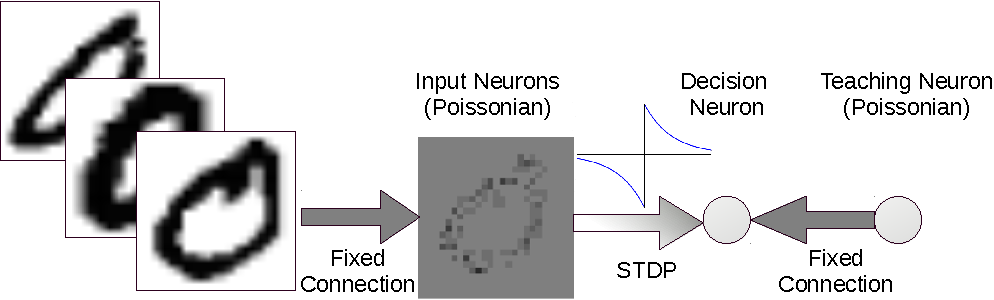
\includegraphics[width=0.48\textwidth]{images/training.pdf}
		} \\

	\centering
	
	\subfloat[Testing model of the spiking neural network.]{
		\label{Fig:test}
		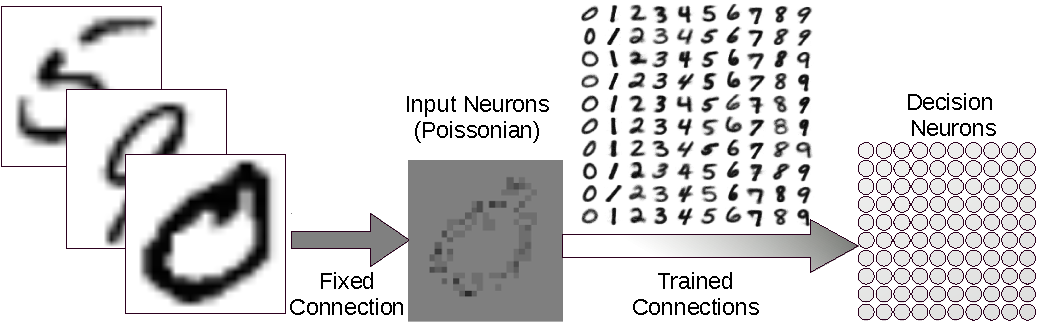
\includegraphics[width=0.48\textwidth]{images/testing.pdf}
		}
		
	\caption{The training and testing model of the two-layered spiking neural network.}
	\label{fig:model}
\end{figure} 



Both the training and testing exploited the Poissonian subset of the NE15-MNIST dataset.
Because different simulators generate random Poissonian spike trains with various mechanisms, languages and codes, using the same dataset is able to evaluate performance of these simulators without the interference by the non-unified input.
In terms of this case study, the performance of the model was evaluated with both software simulation (on NEST~[\cite{gewaltig2007nest}]) and hardware implementation (on SpiNNaker). 

%\subsection{Description of the data used}
\subsubsection{Training}

There are two layers in the neural network model.
And 28$\times$28 input neurons fully connected to 100 output neurons.
Each output neuron represented a trained template of a digit.
Thus there were 10 templates for each digit.
The firing rate of the input neurons were assigned linearly according to their intensities and normalised with a total firing rate of 2000~$Hz$.
The training set of 60000 hand written digits were firstly classified into 100 classes, 10 classes per digit, using K-means clusters.
Every image was presented 300~$ms$ during training and at the same time a teaching signal of 50~$Hz$ was conveyed to the responding output neuron (1 out of 100) to trigger the learning, see Fig~\ref{Fig:train}.
The trained weights were plotted in align with the input image size in Fig~\ref{Fig:test}.
%\begin{figure}[hbt!]
%	\centering
%	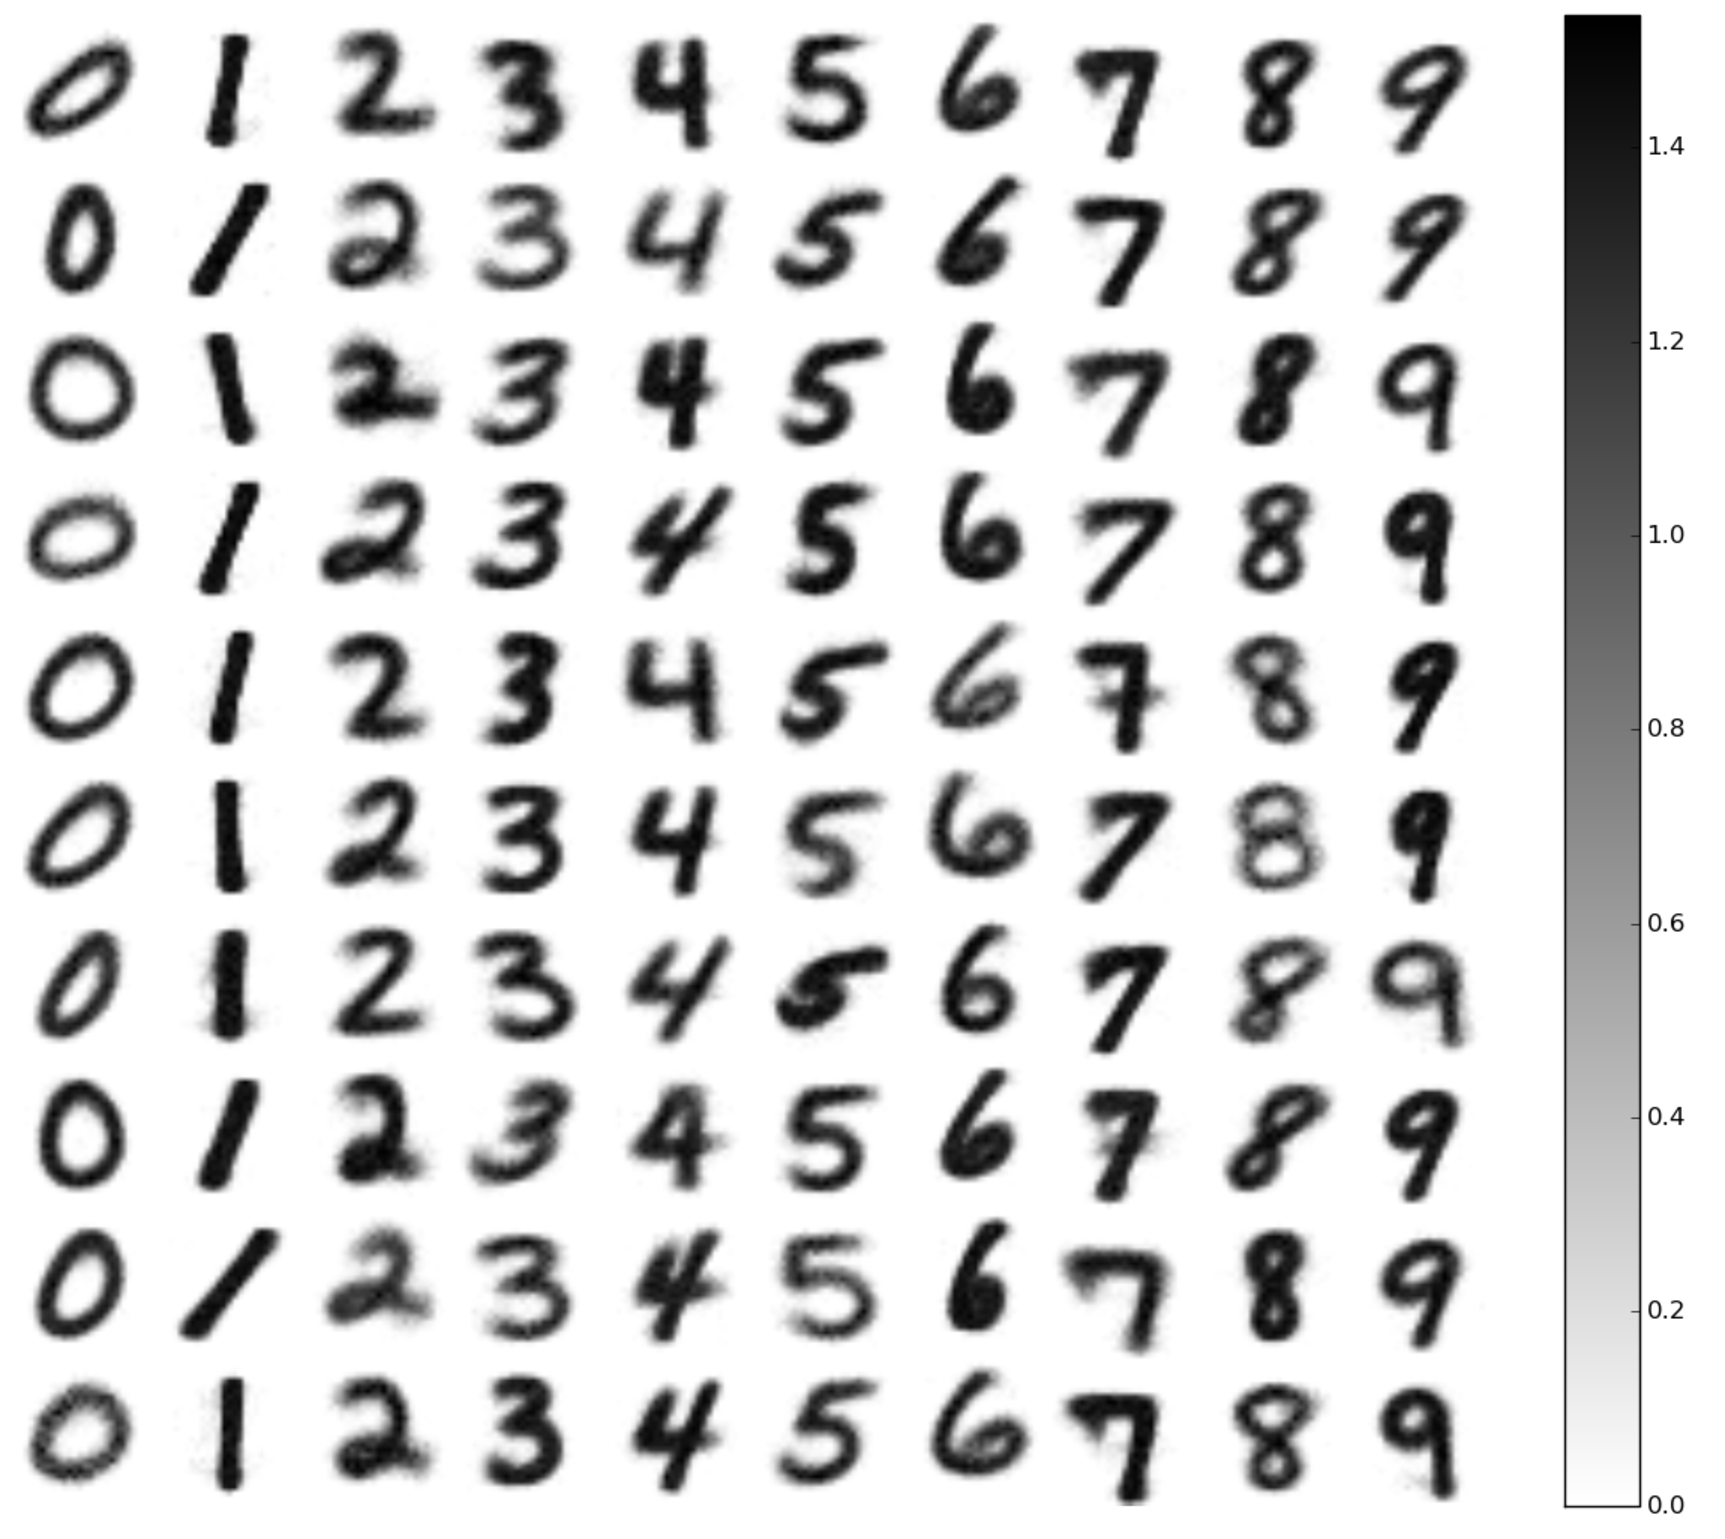
\includegraphics[width=0.48\textwidth]{images/weight_r.pdf}
%	\caption{Trained weights of the synapses from input layer to output neurons.}
%	\label{Fig:weight}
%\end{figure}  



\subsubsection{Testing}
The weights were normalised after training and applied to the same network.
And weak weights (=0) were set to inhibitory connections with an identical strength.
%The output neurons inhibited all the other neurons as a winner take all circuit.
The feed=forward testing network is shown in Fig~\ref{Fig:test}.
Poissonion spike trains are generated with input neurons and conveyed through trained synaptic connections to the decision neurons.
Every testing image was presented 1 second to the network, and the output neuron with the highest firing rate decides.
The accuracy of the recognition reached 82.42\%.%83.14\%.
The recording of the output neurons of a test sequence of digits (4, 1, 1, 0, 9, 3, 1, 9, 4, 6) was shown in the raster plot (Fig~\ref{Fig:output}).
Fig~\ref{Fig:test}.

\begin{figure}[hbt!]
	\centering
	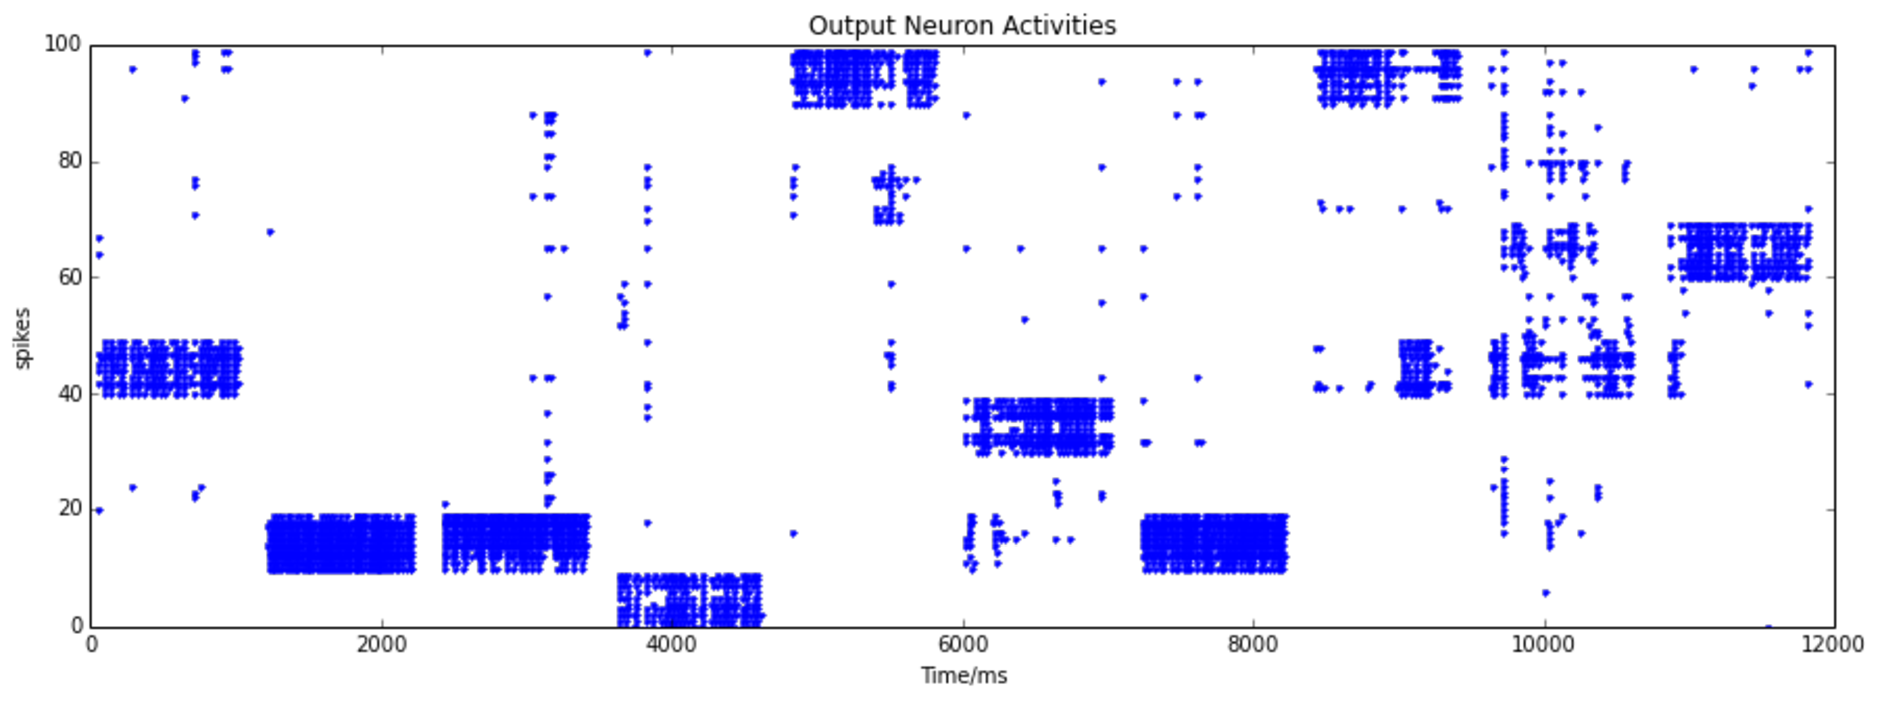
\includegraphics[width=0.48\textwidth]{images/test300-301.pdf}
	\caption{A raster plot of test of a digits sequence.}
	\label{Fig:output}
\end{figure} 
\subsubsection{Evaluation}

\subsection{[Evangelos Stromatias]Case Study II}
\textit{I will use the spiking DBN with the 7 hidden layers, 9 in total. It scores 97\%.}
\subsubsection{Training}
\subsubsection{Testing}
\subsubsection{Evaluation}

\begin{figure}[hbt!]
	\centering
	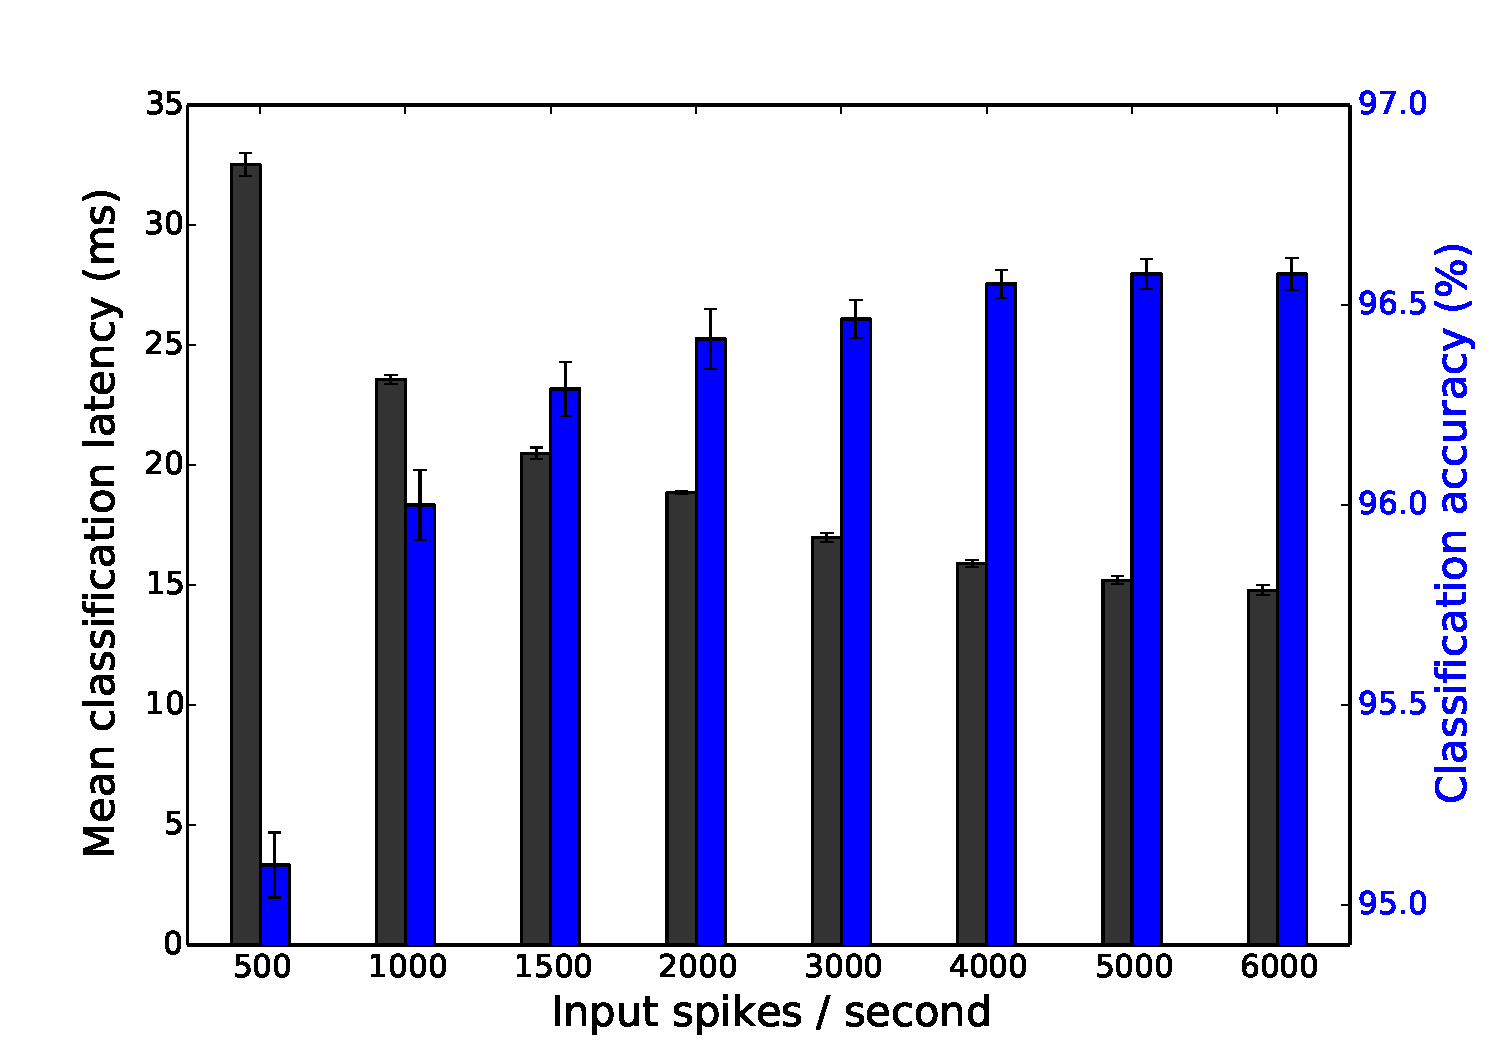
\includegraphics[width=0.48\textwidth]{images/evan/meanCAvsLatencyvsFiringrate_7hlayer.pdf}
	\caption{Classification accuracy as a function of the input firing rates.}
	\label{Fig:rateVSca}
\end{figure} 
